\section{\sys: Data/Memory Protection Methods}

\begin{figure}[t]
	\centering
	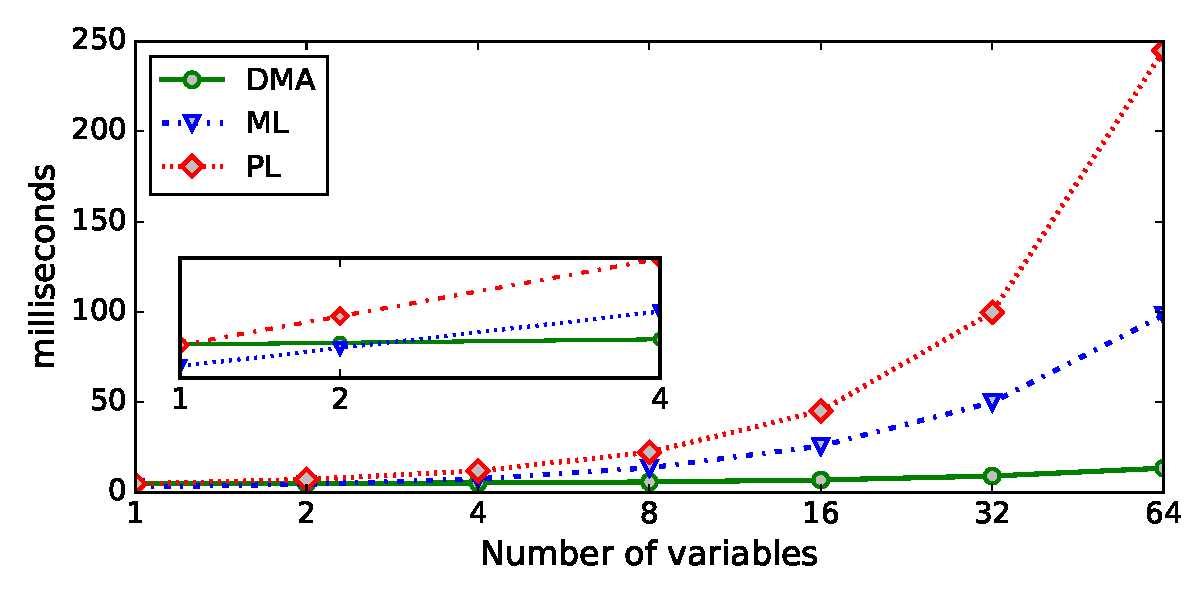
\includegraphics[width=0.8\columnwidth]{figures/iposCommitSize}
	\caption{...}
	\label{fig:virtOperationalBuf}
\end{figure}


\sys data consistency preservation methods are designed with goal of minimal interaction between the CPU and FRAM to reduce energy consumption (see Section~\ref{sec:prelResults}). These data/memory protection methods enables \sys to tolerate arbitrary number of power failures. 

	\subsubsection{Virtualized Operational Buffer}

		\begin{algorithm}[t]
			\caption{Virtualized Operational Buffer}
			\label{algo:virtuBufWrite}
			\scriptsize
			%\small
			\begin{algorithmic}[1]
				\State $var \in \text{\{global variables\}} $ 
				\State \label{lst:virtuBufWrite:line:begin}\Call{Virtual Task()}{} 
				\While { \textit{executing} } \Comment{Execution stage}
					\State $var$  $\rightarrow$ \textsf{volatile buffer} \label{lst:virtuBufWrite:line:output}
					\If { $var$  in \textsf{ volatile buffer} }				\label{lst:virtuBufWrite:line:inputBegin}
							\State $var$  $\leftarrow$  \textsf{volatile buffer} 
						\Else 
							\State $var$  $\leftarrow$  \textsf{FRAM}		\label{lst:virtuBufWrite:line:inputEnd}
						\EndIf

					\If {power interrupts}
						\State back to \ref{lst:virtuBufWrite:line:begin}
					\EndIf
				\EndWhile

				\While{  $\textsf{volatile buffer}\not=\emptyset$  } \label{lst:virtuBufWrite:line:commitBegin} \Comment{ First phase commit}
					\State \textsf{volatile buffer} $\rightarrow$  \textsf{persistent buffer}
					\If {power interrupts}
						\State discard \textsf{persistent buffer}
						\State back to  \ref{lst:virtuBufWrite:line:begin} 
						\State   \label{lst:virtuBufWrite:line:commitEnd}
					\EndIf
				\EndWhile 

				\While{ $\textsf{persistent buffer}\not=\emptyset$ } \label{lst:virtuBufWrite:line:SecCommitBegin} \Comment{Second phase commit}
					\State \textsf{persistent buffer} $\rightarrow$ FRAM 
					\If {power interrupts}
						\State Continue
					\EndIf
				\EndWhile 
				\State     \label{lst:virtuBufWrite:line:SecCommitEnd}
				\State return
			\end{algorithmic}
		\end{algorithm}


		Since accessing FRAM is more energy expensive and slower than accessing SRAM, preventing frequent access to FRAM (i.e. during looping operations) is desirable. Therefore, the first proposed protection method utilizes a volatile buffer that holds temporary all the outputs of a virtual task (see Algorithm~\ref{algo:virtuBufWrite} line~\ref{lst:virtuBufWrite:line:output}). Consequently, a virtual task must first attempt to read a global variable from the volatile buffer before trying to obtain the value from the non-volatile memory (see Algorithm~\ref{algo:virtuBufWrite} lines~\ref{lst:virtuBufWrite:line:inputBegin}-\ref{lst:virtuBufWrite:line:inputEnd}) to ensure a correct execution progress and the consistency of the memory. Once the execution of a virtual task is done, the first phase of the commit process is started by copying the volatile buffer to a persistent buffer (see Algorithm~\ref{algo:virtuBufWrite} lines~\ref{lst:virtuBufWrite:line:commitBegin}-\ref{lst:virtuBufWrite:line:commitEnd}). If the power is interrupted the persistent buffer must be discarded and the execution must start again from the beginning of the virtual task. In another words, the first phase commit must be performed atomically to preserve the consistency of the output of a virtual task. The second phase commit is a power failure immune precess that is responsible for distributing the global variables to their final locations and make the non-volatile memory consistent and synchronized with the computation progress (see Algorithm~\ref{algo:virtuBufWrite}lines~\ref{lst:virtuBufWrite:line:SecCommitBegin}-\ref{lst:virtuBufWrite:line:SecCommitEnd}).


	\paragraph{Virtualized Operational Buffer: Implementation} 

		We implement a reference implementation of \sys that uses virtualized Operational buffer to protect the data against power failure. 
		\paragraph{Virtual Buffer}
			We realized the virtaulzed buffer as a volatile hashed table of linked lists. The hashing technique was chosen to reduce the buffer searching time and the linked lists are used to prevent data loss when there is a conflict between multiple variables---If two variables have the same hash value they will occupy the same cell, however, with linked list a new node will be created for each variable to resolve the conflict and protect the data. The hashing function is based on the observation that the virtual addresses of the memory cells have approximately a flat distribution over the memory addressing space and the fact that each entry, of the virtual table, has the address and the value of a variable. As such, by using the least significant bits as an index to access the virtual buffer the hash function distributes its inputs uniformly in the virtual buffer. Accordingly, the linked lists search time, on average, is reduced. 

			Despite the fact that the linked lists reduce the average complexity of searching the virtual buffer significantly, they introduce a number of drawbacks: (i) the linked list data structure introduce a non-negligible memory overhead while it relies on a limited memory section, namely the heap; (ii) traversing the linked list is relatively slow. Therefore, we re-implemented the virtual buffer, after observing that most of the global variables have the same most significant bits, as a bigger hashed table that does not allow entries conflict. To eliminate the need for searching the hashed table linearly while committing its entries, we add a new buffer that holds the indices of the occupied cells of the hashed table. This table is of the same length as the hashed table. We can reason about the benefit of this buffer as follows: if we assume that the global variables are evenly divided between the tasks, then this buffer reduces the commit time by a factor equal to the number of tasks.   

		\paragraph{Persistent Buffer}
			The persistent buffer is implemented as static array of tuples, where each tuple holds  the address and the value of a variable. This data structure is very suitable for the second phase commit where each element has to be committed to its finial location. However, the complexity of committing this buffer is of size $O(N)$, where $N$ equals the length of the buffer. Therefore, the size of the buffer can have dramatic effect on the performance of \sys---On one hand, if the size of the buffer is small the buffer overflow problem will be very serious. On the other hand, if the size of the buffer is large \sys will experience a significant performance degradation. However, by observing the type of the information that this buffer holds, namely memory addresses, we can, on average, reduce the complexity of committing this buffer by defining the \emph{effective size} of the buffer to be the size of the buffer up to the first cell that holds an invalid memory address. Moreover, since this buffer is in FRAM which is much bigger than SRAM its size can be relatively big. 

		% \paragraph{Virtualized Operational Buffer: delay analysis}[initial results]

		% \begin{figure}[t]
		% 	\centering
		% 	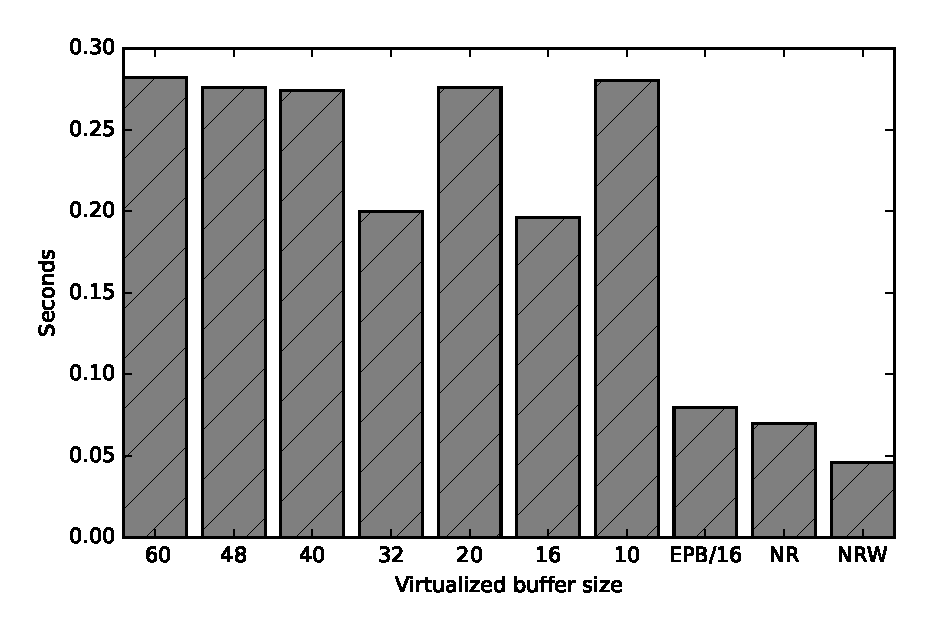
\includegraphics[width=\columnwidth]{figures/virtual_buffer_size.eps}
		% 	\caption{\sys based on virtualized Operational Buffer. It runs the decompression application with different buffer configurarions. EPB: Enhanced Persistent Buffer. NR: no read operation from the buffer. NRW: not read or write operations from the buffer.}
		% 	\label{fig:virtOperationalBuf}
		% \end{figure}

		% 	To analyze the performance of \sys versus the sizes of the virtual buffer and the persistent buffer we setup the following experiment. We let IPOS to run the decompression application---until the data decompression is completely finished---and we capture the execution time using a logic analyzer~\cite{xxx}. The results presented in Fig.~\ref{fig:virtOperationalBuf} show the \sys has its best performance when the virtual buffer size is 16, where the execution time was $\approx$196 ms. 

		% 	All the experiments were done with a persistent buffer of size 100. However, the bar labeled with "EPB/16" in  Fig.~\ref{fig:virtOperationalBuf} shows the effect of the enhanced commit process that uses the buffer effective size instead of the buffer maximum size. We see that the execution time is reduced to $\approx$80 ms. Furthermore, we quantized the overhead of the read operations from the buffer, by eliminating this operation, and the bar labeled with "NR" shows that it cost  $\approx$10 ms. Moreover, the overhead of the read and write operations is $\approx$34 ms as compared to \sys best performance, see the bar labeled with "NRW" in Fig.~\ref{fig:virtOperationalBuf}. 


\subsubsection{ Direct Memory Access Based Protection Method (better name is needed)}
%
	\begin{figure}[t]
		\centering
         \subfloat[The time needed to transfer a block of data using pointers versus Direct Memory Access (DMA).]{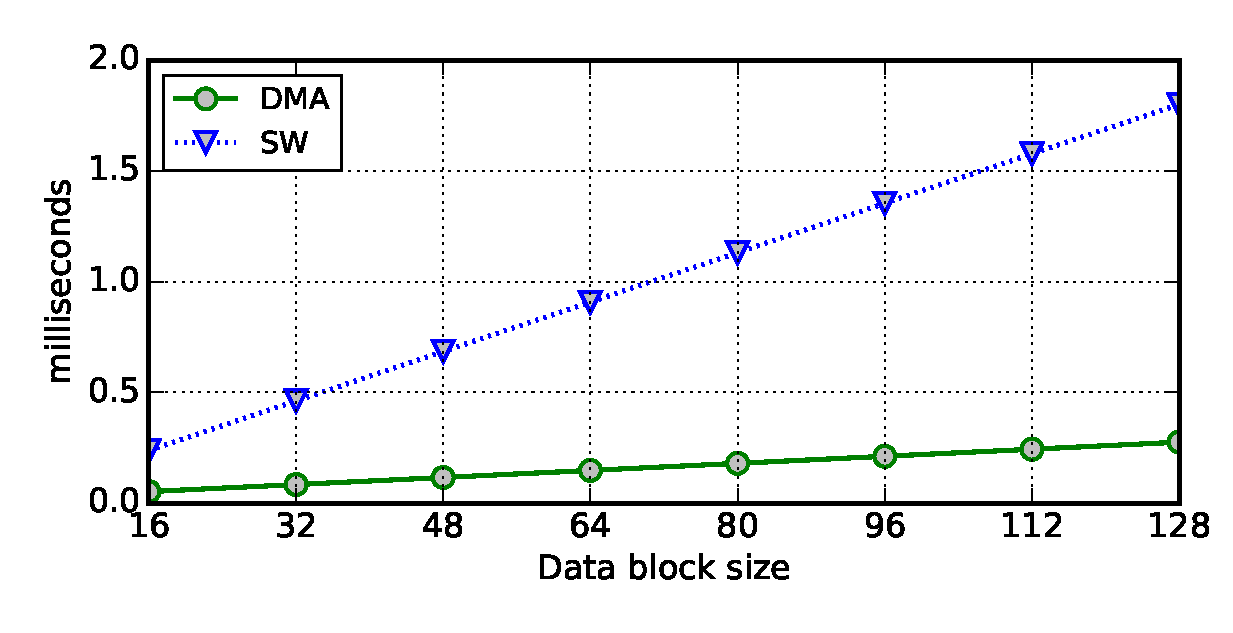
\includegraphics[width=0.48\columnwidth]{figures/dmaSize_time.eps} }
	     \subfloat[The energy needed to transfer a block of data using pointers versus Direct Memory Access (DMA).]{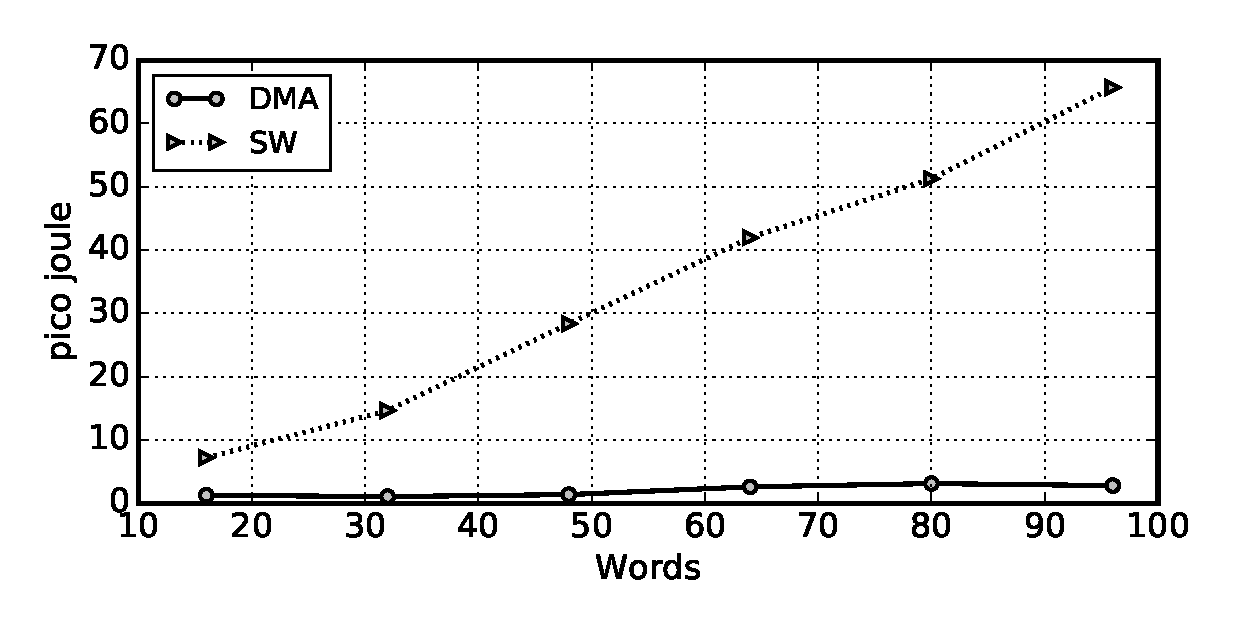
\includegraphics[width=0.48\columnwidth]{figures/energyConsumptionDMA_SW.eps}}
		\caption{Time and energy consumption of moving a block of data from SRAM to FRAM}
		\label{fig:dmaTimeEnergy}
	\end{figure}
%
	Since accessing/updating buffers is more costly than directly accessing FRAM, at least without specialized hardware~\cite{clank}, we introduce the second method to apply the virtualization principle to the Modular Execution Model. This method utilizing the Direct Memory Access (DMA) Module. As Fig.~\ref{fig:dmaTimeEnergy} shows that DMA is much more efficient in transferring a block of data than the conventional (pointer based) way from the energy and time perspectives. 

	This method combines a number of techniques to preserve the persistence and consistency of the data. It backs up the status of the global variables in the non-volatile memory, and double buffers them to guarantee their consistency. Furthermore, on each power up it populates the global variables in the volatile memory from the most recent back up in the non-volatile memory to enable a faster task execution since the task does not need to interact with non-volatile memory which is generally slower and more energy expensive.   

